%%% Local Variables: 
%%% mode: latexTeX-master: t
%%% End: 
\documentclass{beamer}
\usepackage{graphicx}
\usepackage{natbib}
%\usepackage[latin1]{inputenc}
%\usepackage[french]{babel}
%\usepackage[T1]{fontenc}
%\usepackage{verbatim}
\usepackage[normalem]{ulem}
\usepackage{amsmath}
%\usepackage{beamerthemeMadrid}
%\usecolortheme{albatross}
%\usepackage{beamerthemeBoadilla} %pas mal du tout
%\usetheme{JuanLesPins}
\usetheme{Madrid}
%\usetheme{Bergen}
\DeclareMathAlphabet{\mathsl}{OT1}{cmss}{m}{sl}
\usepackage{color}
\usepackage{multicol}
%\usepackage{algorithms/algorithm}
%\usepackage{algorithms/algorithmic}
\usepackage{epsfig}
\usepackage{natbib}
\usepackage{graphicx}              % image
%\usepackage{here}                  % positionement facile des figures
%\usepackage[latin1]{inputenc}      % pour les caracteres accentués
%\usepackage[utf8x]{inputenc}
%\usepackage[francais]{babel}
%\usepackage[cyr]{aeguill}  %package permettant la cesure des mots français
%avec utilisation de font T1 avec bon rendu en pdf
%\usepackage[T1]{fontenc}
%\usepackage{lmodern}
\usepackage{fancyhdr}              %gestion entete /pied de pages
\usepackage{amsmath}
\usepackage{amsfonts}
%include pdf page
\usepackage{pdfpages}
\usepackage{fancybox}
\usepackage{pifont}
%\usepackage{multirow}

\definecolor{brique}{rgb}{0.5,0.2,0.4} 
\definecolor{highlight}{rgb}{1.,0.4,0.}

\newcommand{\RR}{\hbox{\cal I\hspace{-2pt}R}}
\newcommand{\ket}{\right\rangle}       
\newcommand{\bra}{\left\langle}

%\setbeamerfont{frametitle}{series=\bfseries,size=\large,fg=white}
\setbeamerfont{frametitle}{series=\bfseries,size=\large}
\setbeamercolor{structure}{bg=white, fg=brique}

%-------------------------------------------------------------------------------------

\title[hpcscan benchmarks on Shaheen II]{hpcscan version 1.1 \\ Performance benchmarks on Shaheen II (KAUST)}
%\subtitle{}
%\author[Vincent Etienne]{Vincent Etienne}
%\institute[]{XX}

\date[Dec 2020] {\small{December 2020 }}

%-------------------------------------------------------------------------------------

\bibliographystyle{apalike}


\AtBeginSection[ ]
{
\begin{frame}<beamer>
\frametitle{Content}
\tableofcontents[currentsection]
\end{frame}
}

%\AtBeginSubsection[ ]
%{
%\begin{frame}<beamer>
%\frametitle{Content}
%\tableofcontents[currentsection,currentsubsection]
%\end{frame}
%}

%\titlegraphic{\vspace{-0.75cm} \center
%\pgfimage[height=2.cm]{logo/logo_complet.pdf}}

\begin{document}
\scriptsize

\maketitle 

\clearpage

\frame{
\frametitle{Content}
\tableofcontents }

%*************************************************************************************

\section{Introduction}

%*************************************************************************************

%-------------------------------------------------------------------------------------
\frame{
  \frametitle{Introduction}

  All tests in single precision

  Best performance is reported over 10 tries for each cases

  Grids are 3D
  
  }
%-------------------------------------------------------------------------------------

%*************************************************************************************

\section{Shaheen II (KAUST)}

%*************************************************************************************

%-------------------------------------------------------------------------------------
\frame{
  \frametitle{Shaheen II (KAUST)}

  \begin{block}{\center Machine Shaheen II / Cray XC40}

  \scriptsize
  \begin{itemize}
  \item Computing nodes Intel Haswell 2.3 Ghz dual socket (16 cores / socket)
  \item RAM 128 GB with Peak memory BW 136.5 GB/s
  \item Peak performance Single Prec. 2.36 TFLOP/s / Double Prec. 1.18 TFLOP/s
  \item Interconnect Cray Aries with Dragonfly topology
    \begin{itemize}
    \item \scriptsize 60 GB/s optical links between groups
    \item \scriptsize 8.5 GB/s copper links between chassis
    \item \scriptsize 3.5 GB/s backplane within a chassis
    \item \scriptsize 5 GB/s PCIe from node to Aries router
    \end{itemize}
  \end{itemize}

  \end{block}

  \begin{figure}
    \begin{center}
      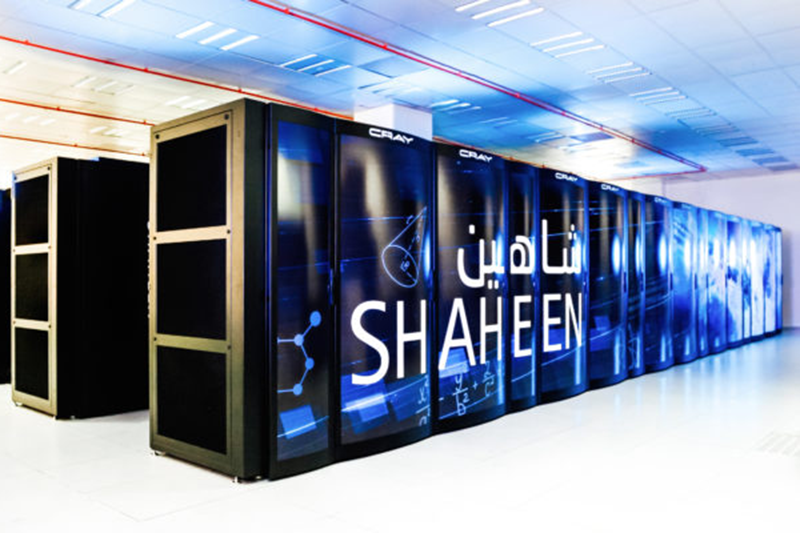
\includegraphics[width=0.5 \textwidth]{./Images/Shaheen-II.png}
    \end{center}
  \end{figure}
}

%*************************************************************************************

\section{Test Case Memory}

%*************************************************************************************

%-------------------------------------------------------------------------------------
\frame{
  \frametitle{Test Case Memory - Description}

  \begin{block}{\center Benchmark objective}
    Measure GByte/s and GPoint/s for
    \begin{itemize}
    \item Fill grid (W = coef)
    \item Copy grid (W = U)
    \item Add grids (W = U + V)
    \item Multiply grids (W = U * V)
    \item Add and update grids (W = W + U)
  \end{itemize}
  \end{block}

  \begin{block}{\center Benchmark configuration}
    \begin{itemize}
    \item Scalability on 1 node with 1 to 32 threads
    \item Baseline kernel
    \item Grid size 4 GB (1000 x 1000 x 1000 points)
    \item Reproduce results with \texttt{./script/testCase\_Memory/hpcscanMemory.sh}
    \item Elapsed time about 4 minutes
    \end{itemize}
  \end{block}
}

%-------------------------------------------------------------------------------------
\frame{
  \frametitle{Test Case Memory - Results \footnote{\scriptsize \textcolor{blue}{Updated Dec 22, 2020}} }

  \begin{figure}
    \begin{center}
      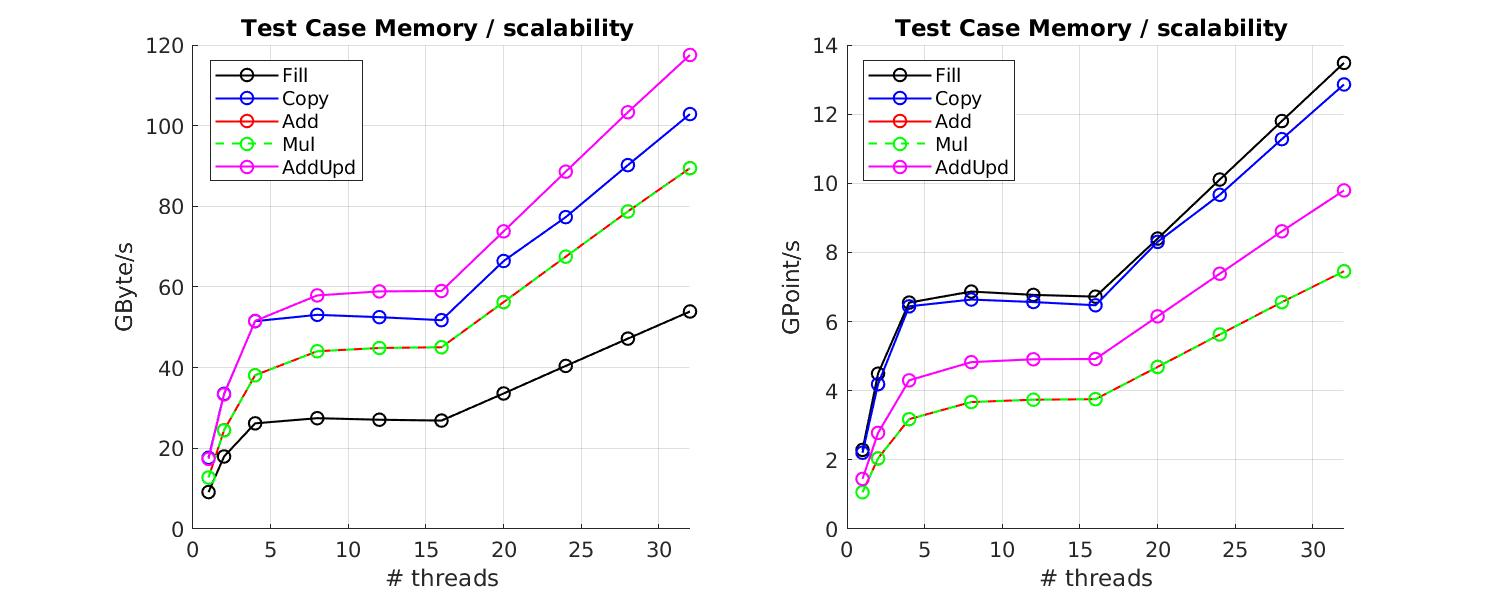
\includegraphics[width=1.0 \textwidth]{../../script/testCase_Memory/hpcscanMemoryShaheen.jpg}
    \end{center}
  \end{figure}
}

%*************************************************************************************

\section{Test Case Grid}

%*************************************************************************************

%-------------------------------------------------------------------------------------
\frame{
  \frametitle{Test Case Grid - Description}

  \begin{block}{\center Benchmark objective}
    Measure GByte/s and GPoint/s for
    \begin{itemize}
    \item Fill grid (U = coef)
    \item Max. diff (U-V)
    \item L1 norm between U and V
    \item Sum Abs(U) \& Sum Abs(U-V)
    \item Get max. \& Get min. grid U
    \item Update pressure (used in propagator)
    \item Boundary condition (free surface at all edges)
  \end{itemize}
  \end{block}

  \begin{block}{\center Benchmark configuration}
    \begin{itemize}
    \item 1 node with 32 threads
    \item Baseline kernel
    \item 2 grid sizes
      \begin{itemize}
      \item \tiny Small size 500 MB (500 x 500 x 500 points)
      \item \tiny Medium size 4 GB (1000 x 1000 x 1000 points)
      \end{itemize}
    \item Reproduce results with \texttt{./script/testCase\_Grid/hpcscanGrid.sh}
    \item Elapsed time less than 1 minute
    \end{itemize}
  \end{block}
  
}

%-------------------------------------------------------------------------------------
\frame{
  \frametitle{Test Case Grid - Results \footnote{\scriptsize \textcolor{blue}{Updated Dec 23, 2020}} }

  \begin{figure}
    \begin{center}
      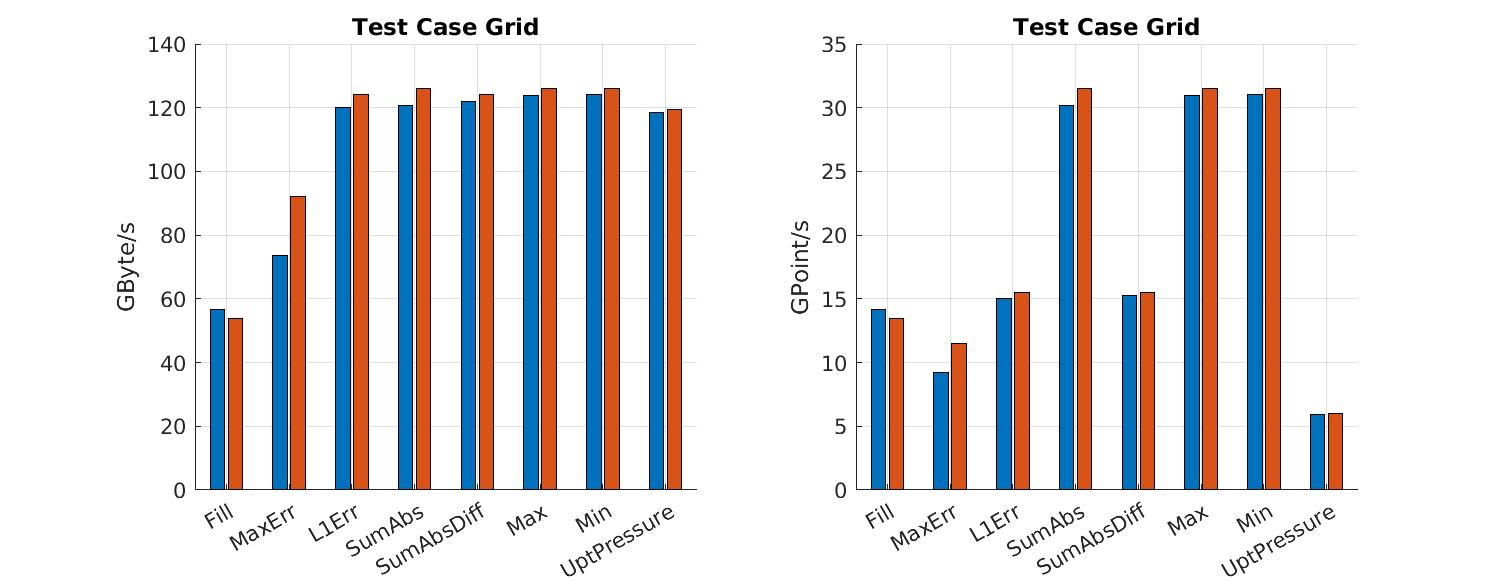
\includegraphics[width=1.0 \textwidth]{../../script/testCase_Grid/hpcscanGridShaheen.jpg}
    \end{center}
  \end{figure}

  Blue small grid / Red medium grid
  
  ApplyBoundaryCondition performs at 713/846 GBytes (89/105 Gpoint/s)
}

%*************************************************************************************

\section{Test Case Comm}

%*************************************************************************************

%-------------------------------------------------------------------------------------
\frame{
  \frametitle{Test Case Comm - Description}

  \begin{block}{\center Benchmark objective}
    Measure GByte/s and GPoint/s for
  
    \vspace{0.25cm}
    MPI point to point communication
    \begin{itemize}
    \item Send with MPI\_Send from proc X to proc 0 (Half-duplex BW)
    \item Send and receive with MPI\_Sendrecv between proc X and proc 0 (Full-duplex BW)
    \end{itemize}

    MPI collective communication
    \begin{itemize}
    \item Exhange of halos used in FD kernel with MPI\_Sendrecv
    \item Domain decomposition with N1 x N2 x N3 subdomains
    \end{itemize}
  \end{block}

  \begin{block}{\center Benchmark configuration}
    \begin{itemize}
    \item 8 nodes with 32 threads
    \item Baseline kernel
    \item Grid size 4 GB (1000 x 1000 x 1000 points)
    \item Subdomain decomposition: 1x4x2 / 1x2x4 \& 2x2x2
    \item Reproduce results with \texttt{./script/testCase\_Comm/hpcscanComm.sh}
    \item Elapsed time less than 1 minute
    \end{itemize}
  \end{block}
}


%-------------------------------------------------------------------------------------
\frame{
  \frametitle{Test Case Comm - Results \footnote{\scriptsize \textcolor{blue}{Updated Sep 19, 2020}} }

  {\tiny
  \begin{table}
    \caption{\scriptsize Bandwidth GB/s}
    \label{table_comm}
    \begin{tabular}{@{}ccccccc}
      MPI\#1 & MPI\#2 & Send & Sendrecv & Halo exch. & Comm. size & Subdomains \\
      \hline
      0 & 1 & 8.5 & 15.3 & -    & 47 MB  & - \\
      0 & 2 & 8.3 & 15.3 & -    & 47 MB  & - \\
      0 & 3 & 8.6 & 15.3 & -    & 47 MB  & - \\
      0 & 4 & 8.5 & 15.3 & -    & 47 MB  & - \\
      0 & 5 & 8.2 & 15.3 & -    & 47 MB  & - \\
      0 & 6 & 8.5 & 15.3 & -    & 47 MB  & - \\
      0 & 7 & 8.6 & 15.3 & -    & 47 MB  & - \\
      All & All & -    & -   & 5.0  & 128 MB & 1 4 2 \\
      All & All & -    & -   & 5.1  & 128 MB & 1 2 4 \\
      All & All & -    & -   & 2.0  & 96 MB  & 2 2 2 \\
    \end{tabular}
  \end{table}
  }

}

%*************************************************************************************

\section{Test Case FD\_D2}

%*************************************************************************************

%-------------------------------------------------------------------------------------
\frame{
  \frametitle{Test Case FD\_D2 - Description}

  \begin{block}{\center Benchmark objective}
    Measure GByte/s, GPoint/s \& Gflop/s for
    \begin{itemize}
    \item Computation of second order derivatives with finite-difference stencil
    \item Directionnal derivatives
      \begin{itemize}
      \item {\tiny Axis 1, $W = \partial^2_{x1} (U)$}
      \item {\tiny Axis 2, $W = \partial^2_{x2} (U)$}
      \item {\tiny Axis 3, $W = \partial^2_{x3} (U)$}
      \end{itemize}
    \item Laplacian $W = \Delta (U)$
    \item Stencil orders 2, 4, 8, 12 \& 16
    \end{itemize}
    
  \end{block}

  \begin{block}{\center Benchmark configuration}
    \begin{itemize}
    \item 1 node with 32 threads
    \item 2 test modes
      \begin{itemize}
      \item \tiny Baseline
      \item \tiny CacheBlk
      \end{itemize}
    \item Grid size 4 GB (1000 x 1000 x 1000 points)
    \item Reproduce results with \texttt{./script/testCase\_FD\_D2/hpcscanFD\_D2.sh}
    \item Elapsed time about 2 minutes
    \end{itemize}
  \end{block}
}

%-------------------------------------------------------------------------------------
\frame{
  \frametitle{Test Case FD\_D2 - Results \footnote{\scriptsize \textcolor{blue}{Updated Dec 24, 2020}} }

  \begin{figure}
    \begin{center}
      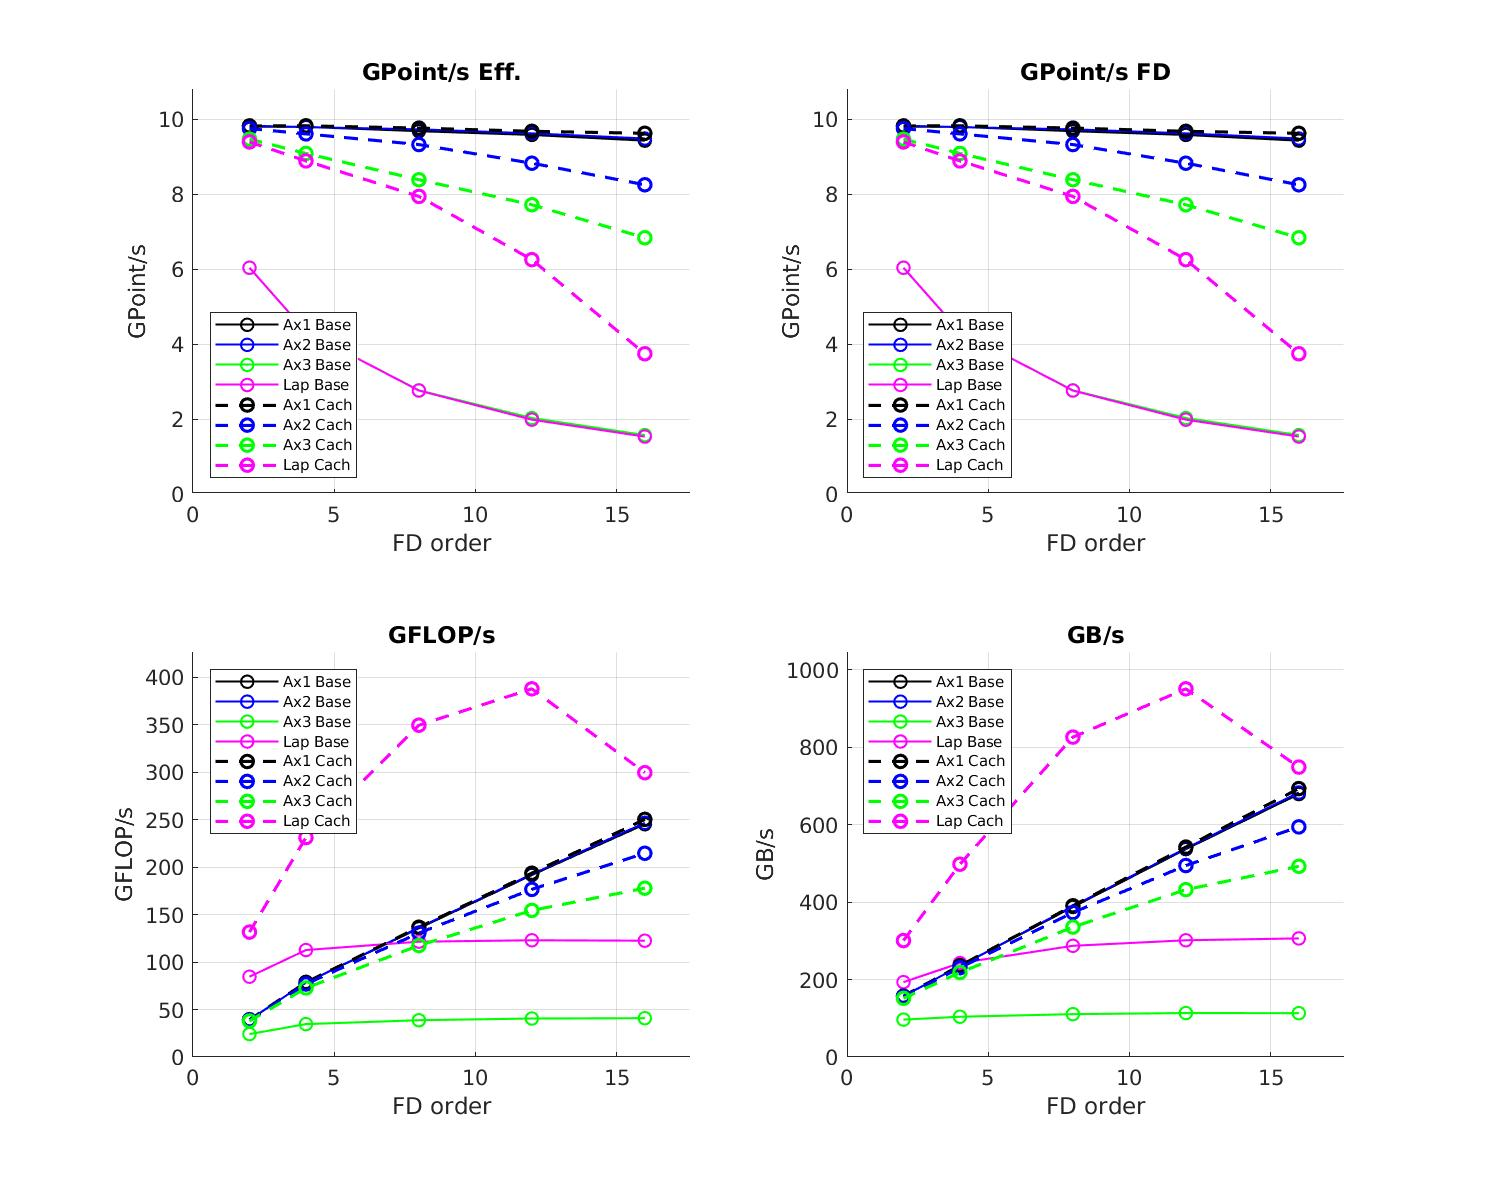
\includegraphics[width=0.8 \textwidth]{../../script/testCase_FD_D2/hpcscanFD_D2Shaheen.jpg}
    \end{center}
  \end{figure}
}

%*************************************************************************************

\section{Test Case Propa}

%*************************************************************************************

%-------------------------------------------------------------------------------------
\frame{
  \frametitle{Test Case FD\_D2 - Description}

  \begin{block}{\center Benchmark objective}
    Measure GByte/s, GPoint/s \& Gflop/s for
    \begin{itemize}
    \item Acoustic wave propagator
    \item Stencil orders 2, 4, 8, 12 \& 16
    \item Time step 1, 0.5 \& 0.1 of stability time step
    \end{itemize}
    
  \end{block}

  \begin{block}{\center Benchmark configuration}
    \begin{itemize}
    \item 1 node with 32 threads
    \item Test mode CachBlk
    \item 2 propagator implementations
      \begin{itemize}
      \item \tiny Ac2Standard
      \item \tiny Ac2SplitComp
      \end{itemize}
    \item Grid size from $500^3$ (500 MB) to $1000^3$ (4 GB)
    \item Reproduce results with \texttt{./script/testCase\_PropaparamAnalysis/hpcscanPropaParamAnalysis.sh}
    \item Elapsed time about XX minutes
    \end{itemize}
  \end{block}
}

%-------------------------------------------------------------------------------------
\frame{
  \frametitle{Test Case Propa - Results \footnote{\scriptsize \textcolor{blue}{Updated Nov 5, 2020}} }
  
  \begin{figure}
    \begin{center}
      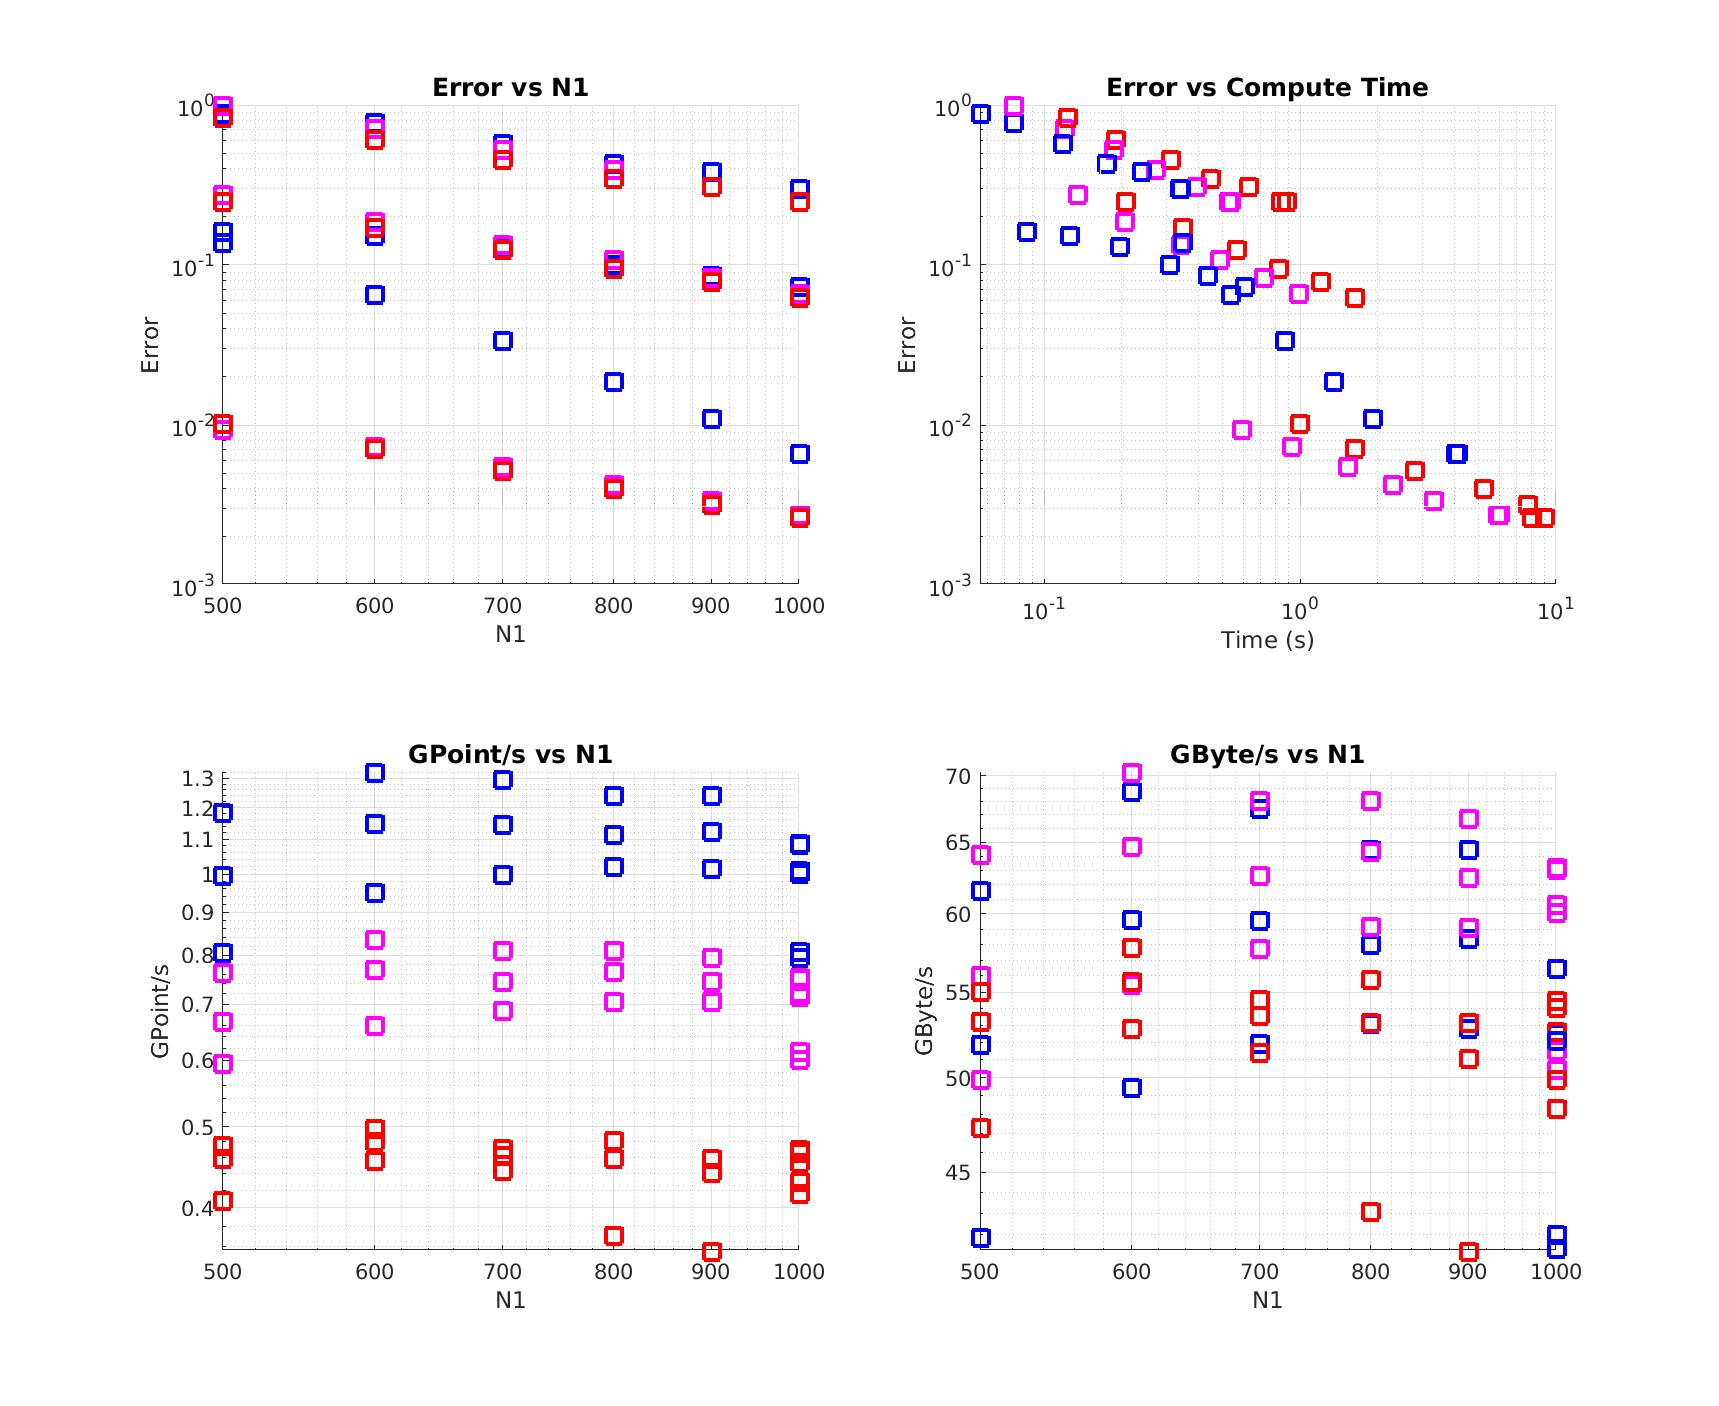
\includegraphics[width=0.6 \textwidth]{./Figures/runMars_AccPerf.jpg}
    \end{center}
  \end{figure}
}

%-------------------------------------------------------------------------------------
\frame{
  \frametitle{Test Case FD\_D2 - Description}

  \begin{block}{\center Benchmark objective}
    Measure GByte/s, GPoint/s \& Gflop/s for
    \begin{itemize}
    \item Acoustic wave propagator
    \item Stencil order 8
    \item Strong and weak scalability
    \end{itemize}
    
  \end{block}

  \begin{block}{\center Benchmark configuration}
    \begin{itemize}
    \item From 1 node to 8 nodes with 32 threads/node
    \item Test mode CachBlk
    \item Propagator implementation Ac2Standard
    \item Strong scalability: Grid size $1000^3$ (4 GB)
    \item Weak scalability: Grid size from 1000x1000x1000 (4 GB) to 1000x4000x2000 (32 GB)
    \item Reproduce results with \texttt{./script/testCase\_strongWeakScalability/hpcscanPropaStrongWeakScalability.sh}
    \item Elapsed time about 7 minutes
    \end{itemize}
  \end{block}
}


%-------------------------------------------------------------------------------------
\frame{
  \frametitle{Test Case Propa - Results \footnote{\scriptsize \textcolor{blue}{Updated Dec 26, 2020}} }

  \begin{figure}
    \begin{center}
      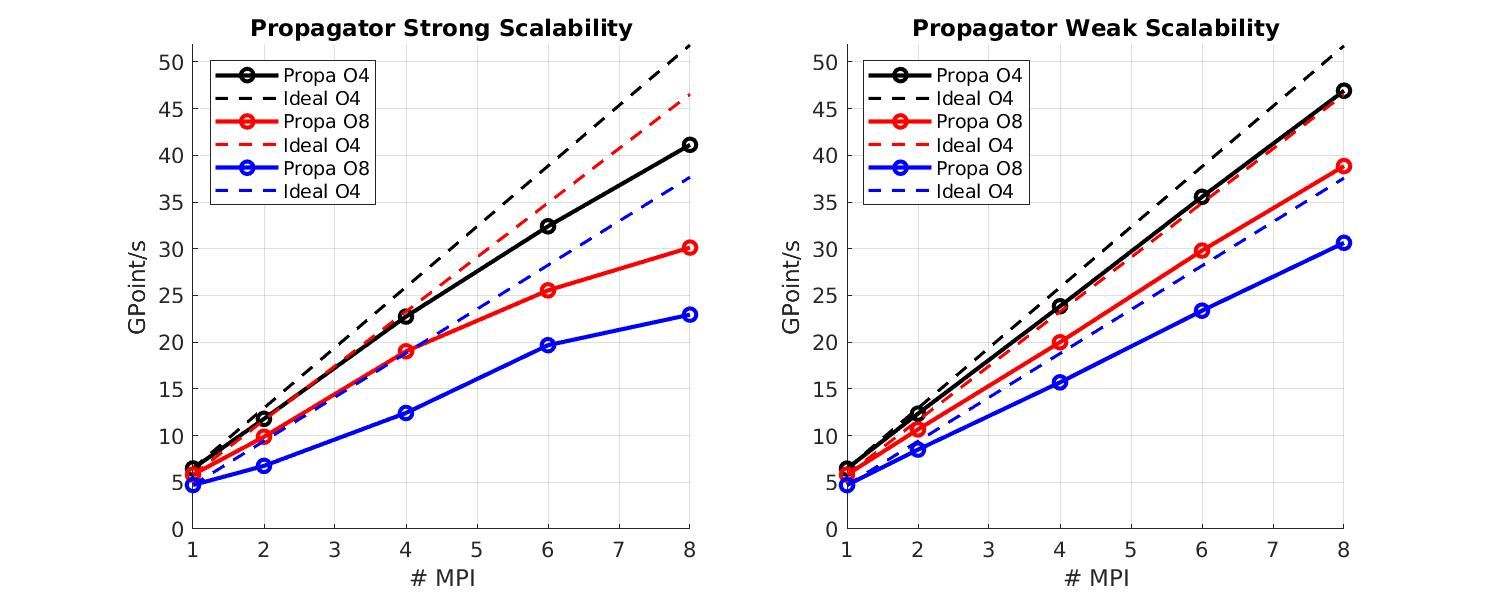
\includegraphics[width=1.0 \textwidth]{../../script/testCase_Propa/strongWeakScalability/hpcscanPropaStrongWeakScalabilityShaheen.jpg}
    \end{center}
  \end{figure}
}

%*************************************************************************************

\section{Summary}

%*************************************************************************************

%-------------------------------------------------------------------------------------
\frame{
  \frametitle{Summary}

  \begin{block}{\center Test Case Memory}
    \begin{itemize}
    \item Measured memory BW between 91 to 122 GB/s (67-90 \% of peak BW)
    \item Low BW 59 GB/s for Fill (43 \% of peak BW)
    \item Multiply (= imaging condition) performs at 7.6 Gpoint/s
    \end{itemize}
  \end{block}

  \begin{block}{\center Test Case Grid}
    \begin{itemize}
    \item L1 Err., Get Min \& Max: 125 GB/s close to peak BW (92 \% Peak Mem. BW)
    \item {Low perf for Fill: 54-58 GB/s (40-43 \% Peak Mem. BW)}
    \item Max Err. 72-91 GB/s (53-67 \% Peak Mem. BW)
    \item Pressure update 6 GPoint/s (120 GB/s, 88 \% Peak Mem. BW)
    \end{itemize}
  \end{block}
  }
%-------------------------------------------------------------------------------------

%-------------------------------------------------------------------------------------
\frame{
  \frametitle{Summary}

  \begin{block}{\center Test Case Comm}
    \begin{itemize}
    \item TO DO
    \end{itemize}
  \end{block}
}
%-------------------------------------------------------------------------------------

%-------------------------------------------------------------------------------------
\frame{
  \frametitle{Summary}
  
  \begin{block}{\center Test Case FD\_D2}
    \begin{itemize}
    \item Large benefit of cache blocking
    \item Significant effect of grid dimnsion and index (very bad performance for n3 without cache blocking)
    \item Min BW 50 GFLOP/s ($\partial^2_{x3}$ O2) = 2 \% peak BW [apparent Mem. BW 150 GB/s]
    \item Max BW 370 GFLOP/s ($\Delta$ O8) = 16 \% peak BW [apparent Mem. BW 900 GB/s]
    \item Apparent Mem. BW 150-900 GB/s (110-660 \% Peak Mem. BW) = shows data in-cache effect
    \item Typical stencils of interest for geophysical applications
      \begin{itemize}
      \item {\scriptsize $\Delta$ O4  BW = 8-10 GPoint/s}
      \item {\scriptsize $\Delta$ O8  BW = 7-9 GPoint/s}
      \item {\scriptsize $\Delta$ O12 BW = 3-5 GPoint/s}
      \end{itemize}
    \item Parallel efficiency with 8 nodes 55 to 86 \% (depends on workload on Shaheen)
    \end{itemize}
  \end{block}
}
%-------------------------------------------------------------------------------------

%-------------------------------------------------------------------------------------
\frame{
  \frametitle{Summary}

  \begin{block}{\center Test Case Propa}
    \begin{itemize}
    \item TO DO
    \end{itemize}
  \end{block}
}
%-------------------------------------------------------------------------------------

%*************************************************************************************

\section{Acknowledgements}

%*************************************************************************************

%-------------------------------------------------------------------------------------
\frame{
  \frametitle{Acknowledgements}
  \begin{itemize}
  \item KAUST ECRC and KSL for access and support on Shaheen II
  \end{itemize}
}

%-------------------------------------------------------------------------------------
%{\tiny{
%\def\newblock{\hskip .11em plus .33em minus .07em}
%\bibliographystyle{apalike}
%\bibliography{./biblioseiscope}
%}}

%\addtocounter{framenumber}{-4}

\end{document}

